This section describes our system data flow by presenting it in different layers. A Client layer allows logging in, which passes data to a Server layer, which Communicates to a Database, and sends data to the lower Client layer, the main portion of the website. Data is sent between this bottom layer and the center Server layer frequently while processing new inputs and outputs.

\begin{figure}[h!]
	\centering
 	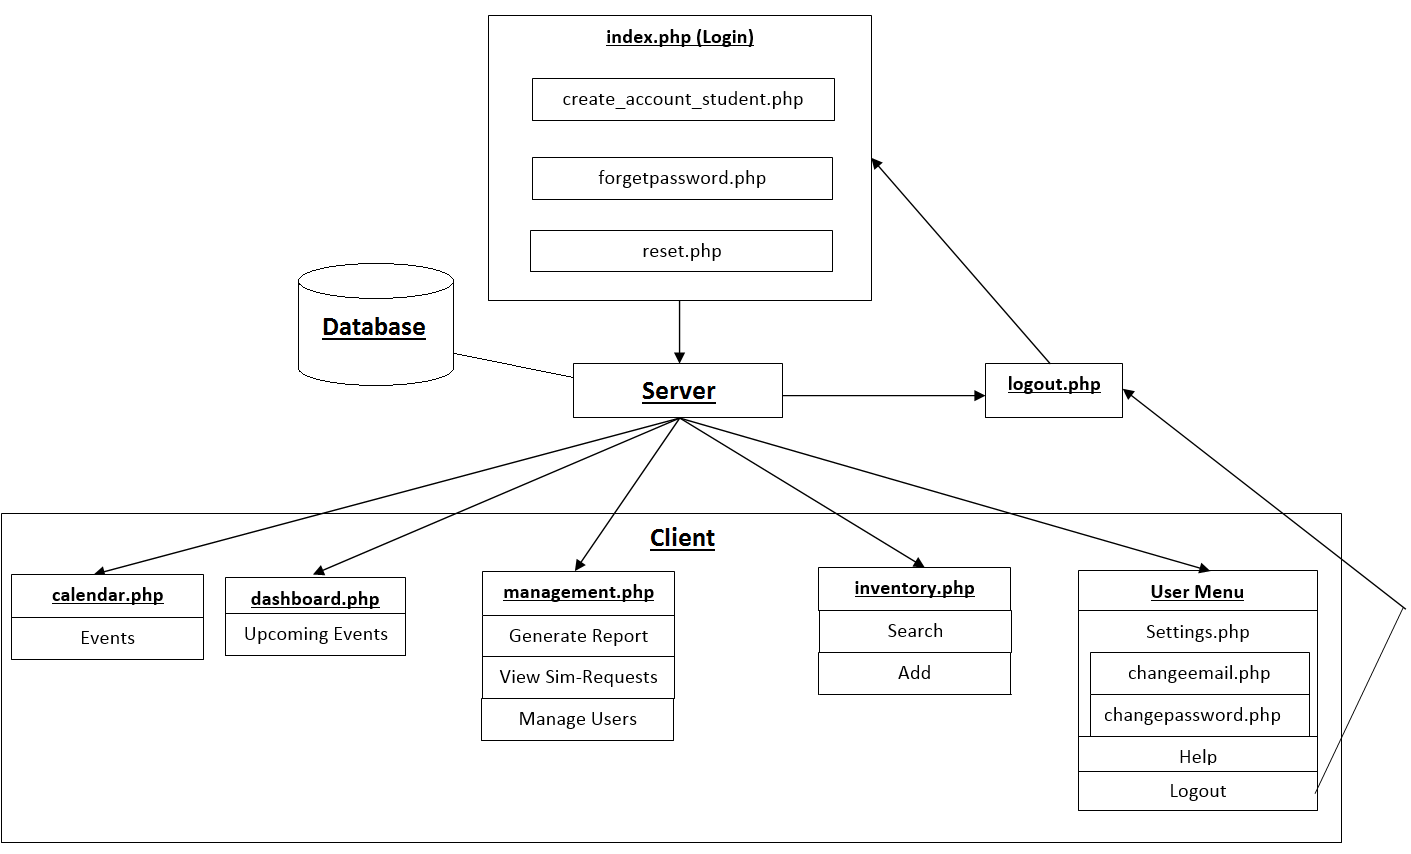
\includegraphics[width=1.0\textwidth]{images/systemoverview}
 \caption{Architectural layer diagram}
\end{figure}

\subsection{Client}
This layer takes input from the user and stores it in the database. It also takes data from the database as well as static content for the webpages from the server in order to display the graphical user interface , along with their data, if they have any. Take the inventory page, for example. The client presses on the inventory tab. The server obtains data from the database, such as what the inventory items are, and the static content for the webpages from the server, and these are linked together to have data loaded on the actual graphical user interface to the client. 

\subsection{Server}
This layer contains static information for the webpages, such as the CSS, Bootstrap, HTML, and php code needed to display the web page, and contains the interface that is needed to link the webpages with the data, if they needed any, as described in the client layer.

\subsection{Data}
This layer stores all the information that needs to be used by users of the website, such as the actual inventory items to be stored in the lab. 